\documentclass[12pt]{amsart}
\usepackage[landscape,margin=1in]{geometry}
\usepackage{graphicx}
\usepackage{wrapfig}
\usepackage{subcaption}


\begin{document}
\thispagestyle{empty}

\begin{figure}
\begin{subfigure}[b]{0.2\textwidth}
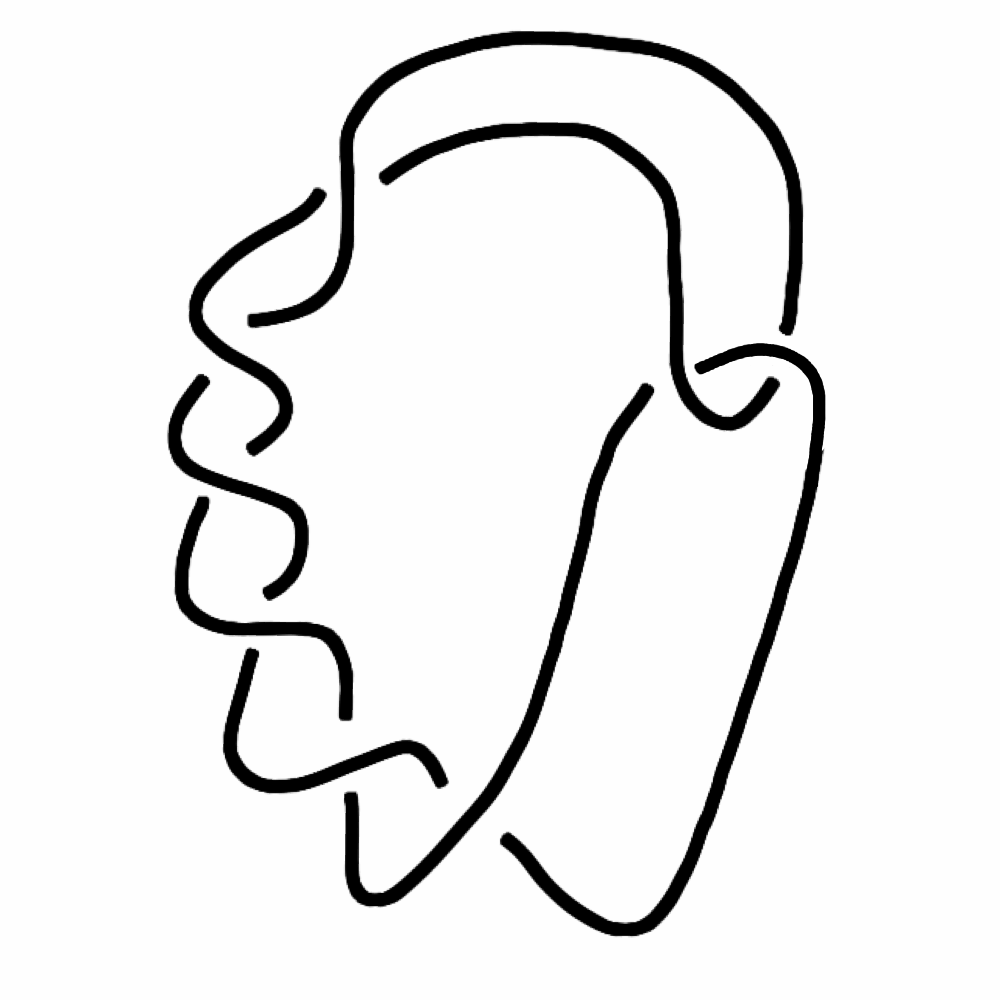
\includegraphics[width=\textwidth]{images/twistknot.png}
\end{subfigure}\qquad
\begin{subfigure}[b]{0.2\textwidth}
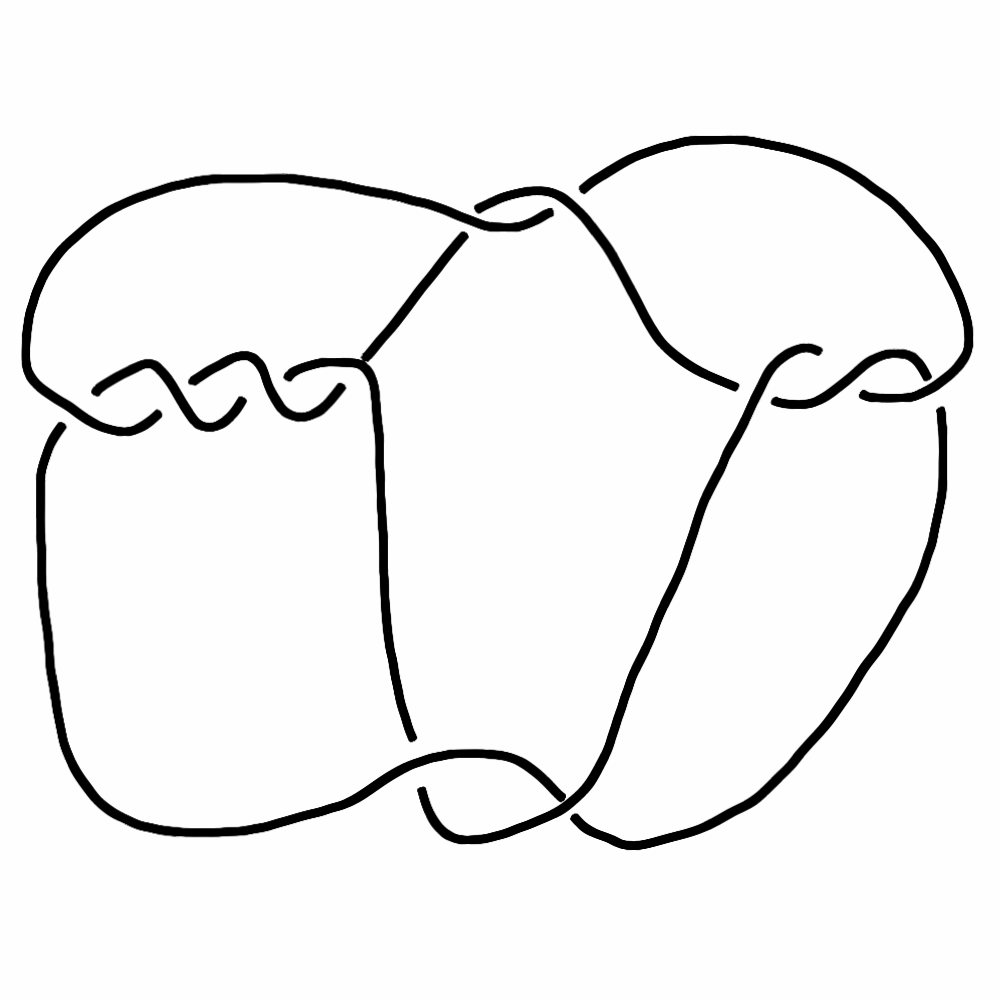
\includegraphics[width=\textwidth]{images/goeritz.png}
\end{subfigure}\qquad
\begin{subfigure}[b]{0.2\textwidth}
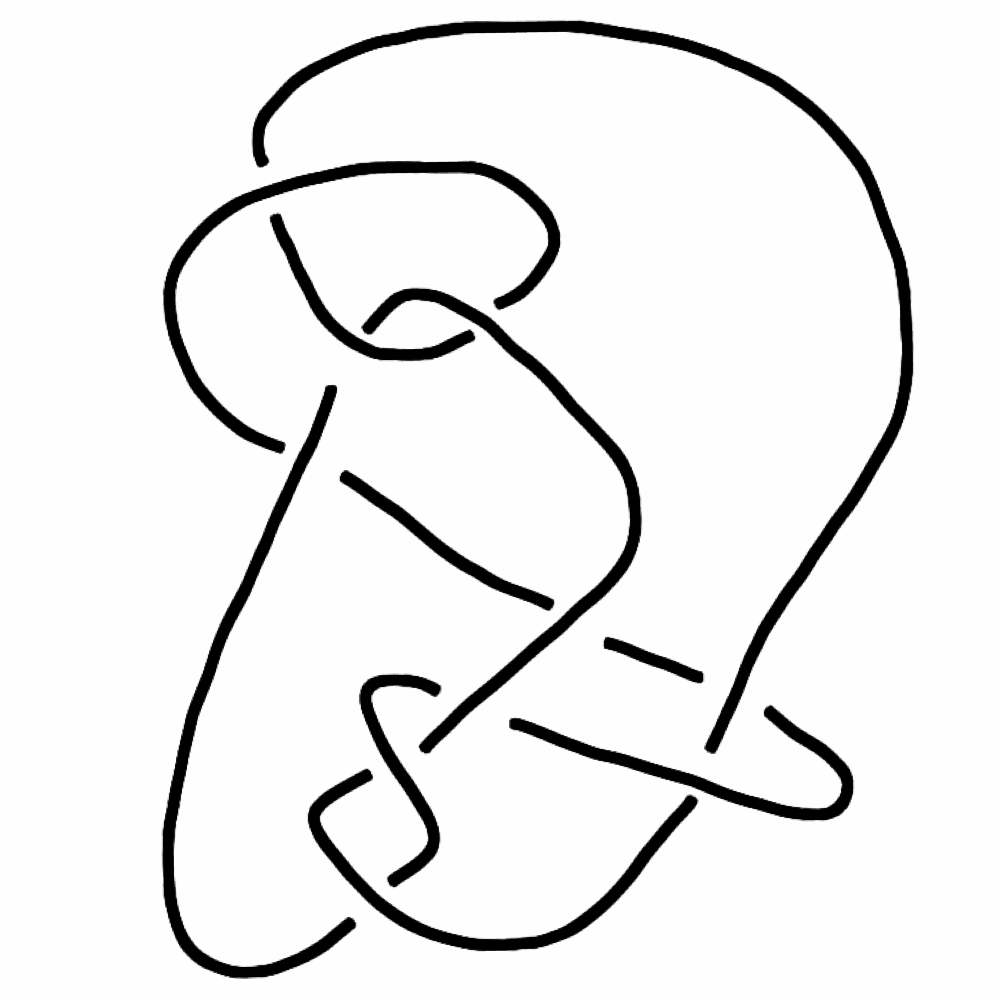
\includegraphics[width=\textwidth]{images/hk-hardunknot.png}
\end{subfigure}\qquad
\begin{subfigure}[b]{0.2\textwidth}
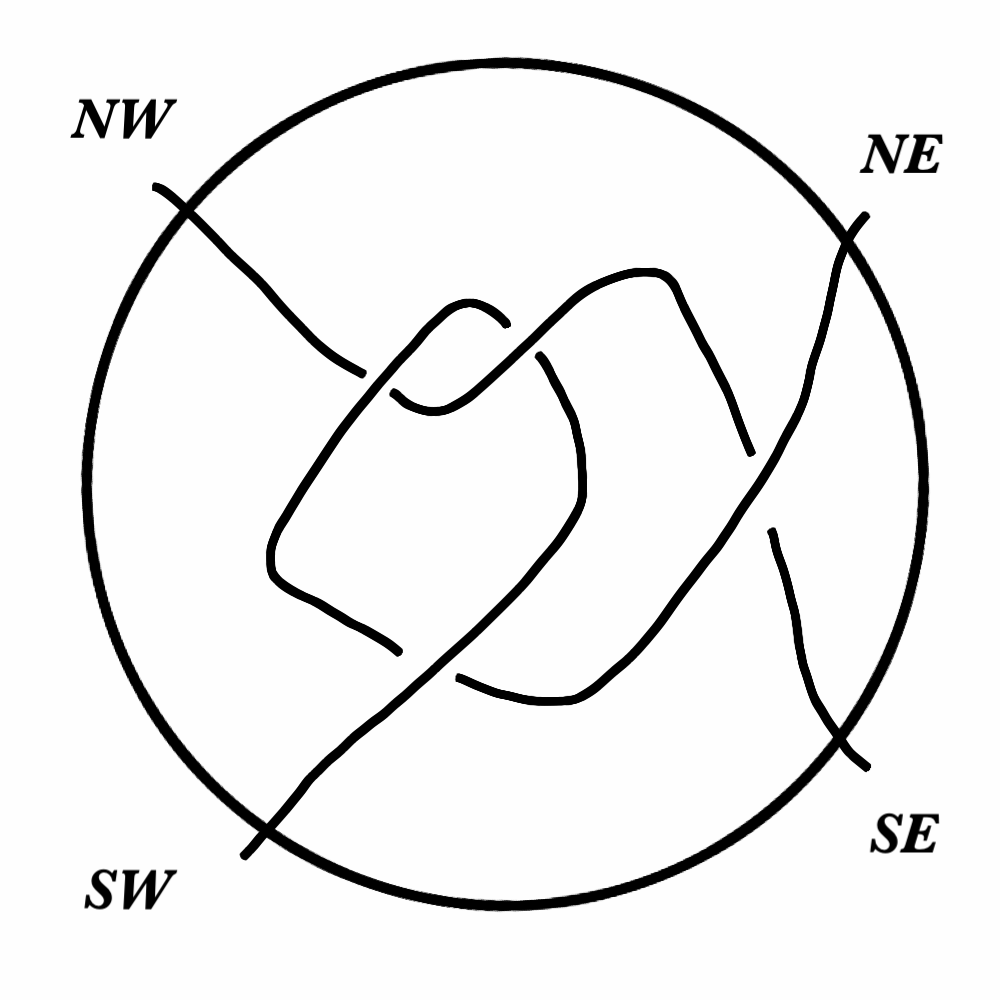
\includegraphics[width=\textwidth]{images/tangle.png}
\end{subfigure}
\end{figure}


\begin{wrapfigure}{L}{0.3\textwidth}
  \centering
  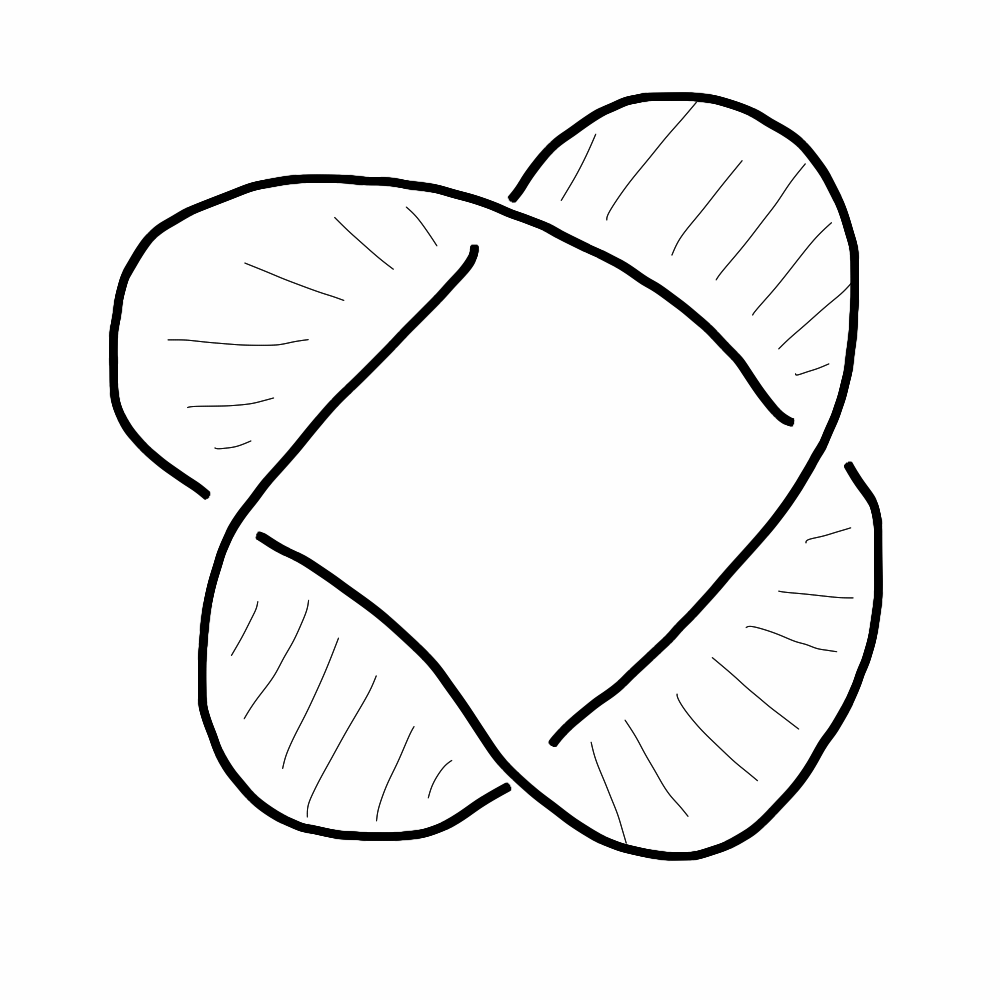
\includegraphics[width=0.29\textwidth]{images/checkerboard.png} 
\end{wrapfigure}



\noindent
\Large
New Course\\
\Huge
Math 4159/5159: \textbf{Knot Theory}\\
\Large
Spring 2017, MWF 10-10:50am\\
\large
Prof Hitchman\\
theron.hitchman@uni.edu\\[.25in]

\noindent
What is a \emph{knot}?\\ 
How can we tell if two knots
are the same or different?\\[.1in]



\begin{figure}[h!]
\begin{subfigure}[b]{0.2\textwidth}
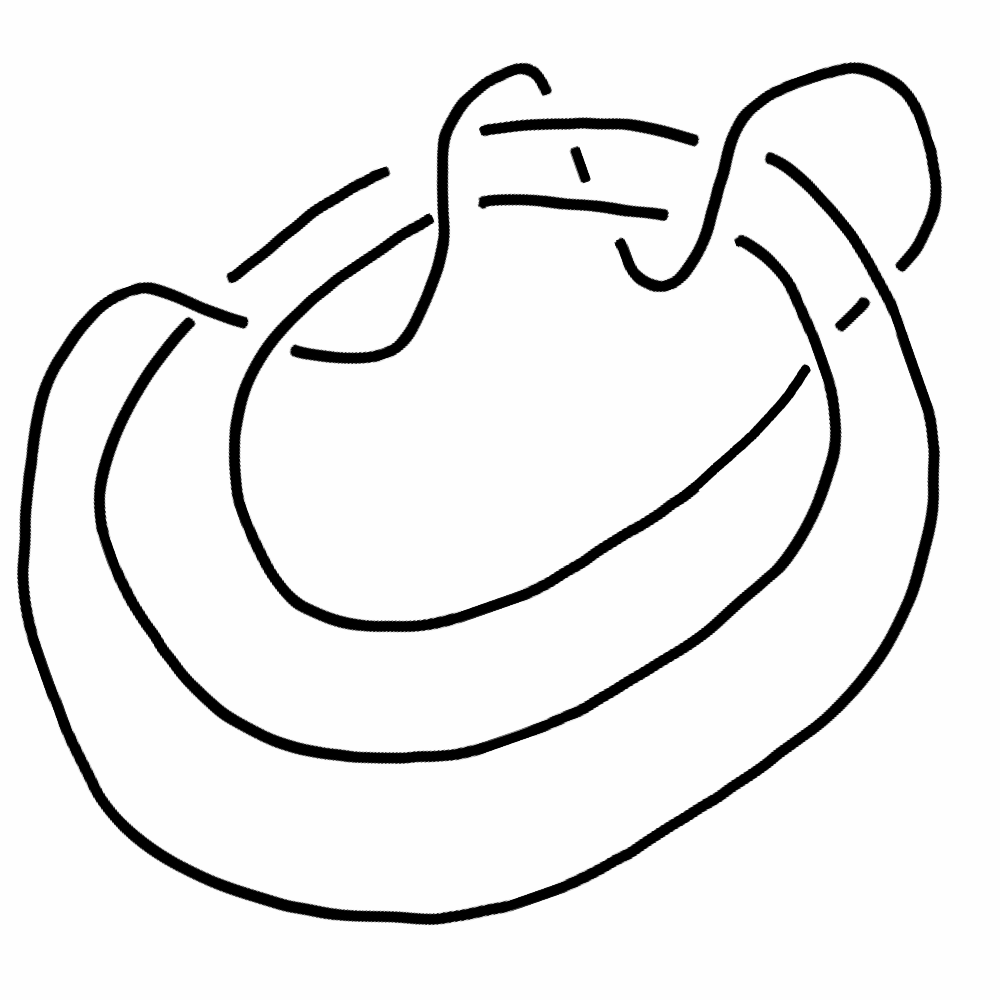
\includegraphics[width=\textwidth]{images/perko10-161.png}
\end{subfigure}\qquad
\begin{subfigure}[b]{0.2\textwidth}
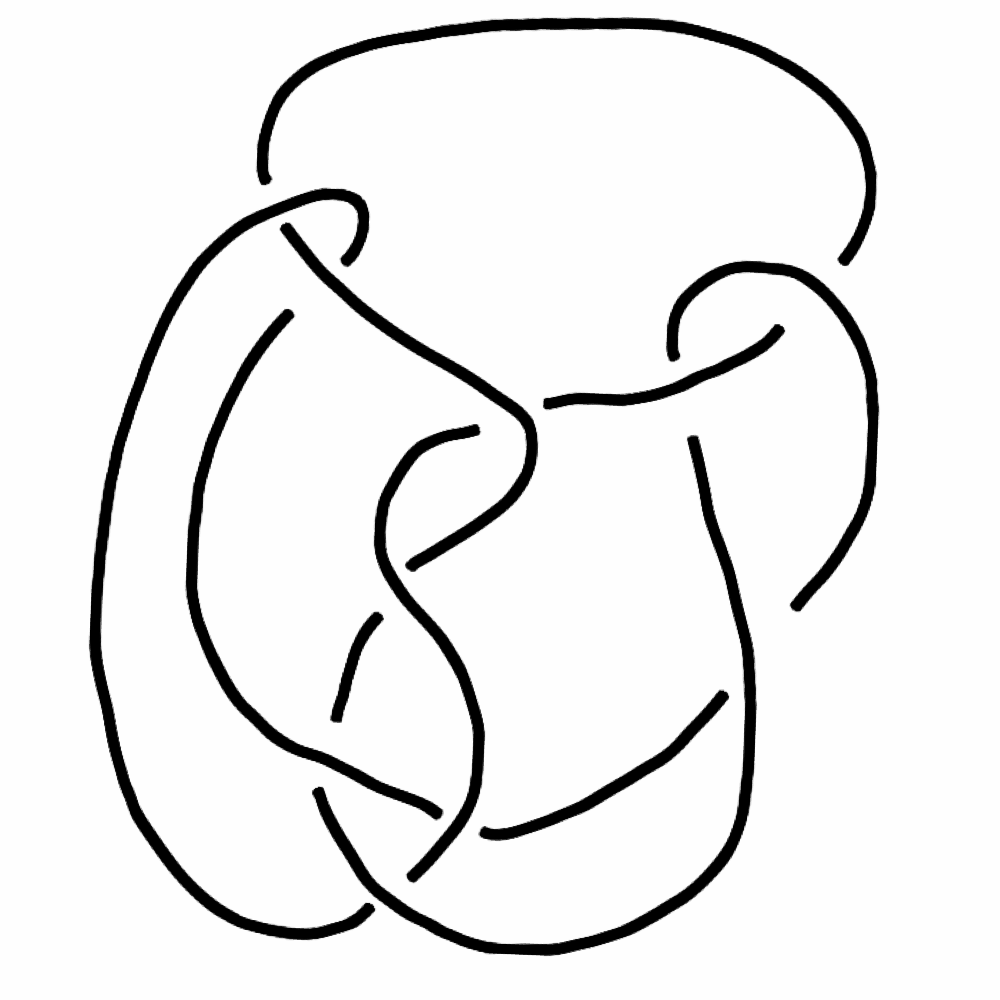
\includegraphics[width=\textwidth]{images/perko10-162.png}
\end{subfigure}\qquad
\begin{subfigure}[b]{0.2\textwidth}
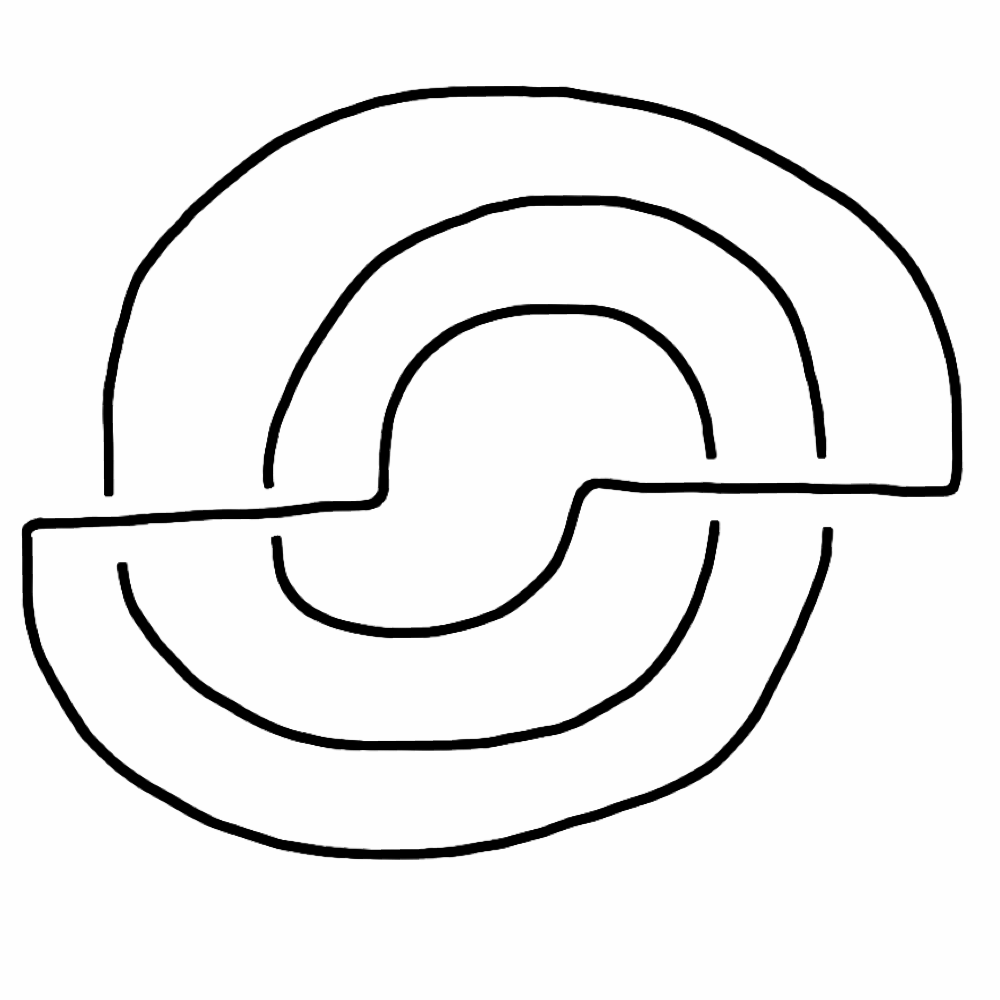
\includegraphics[width=\textwidth]{images/twobridge.png}
\end{subfigure}\qquad
\begin{subfigure}[b]{0.2\textwidth}
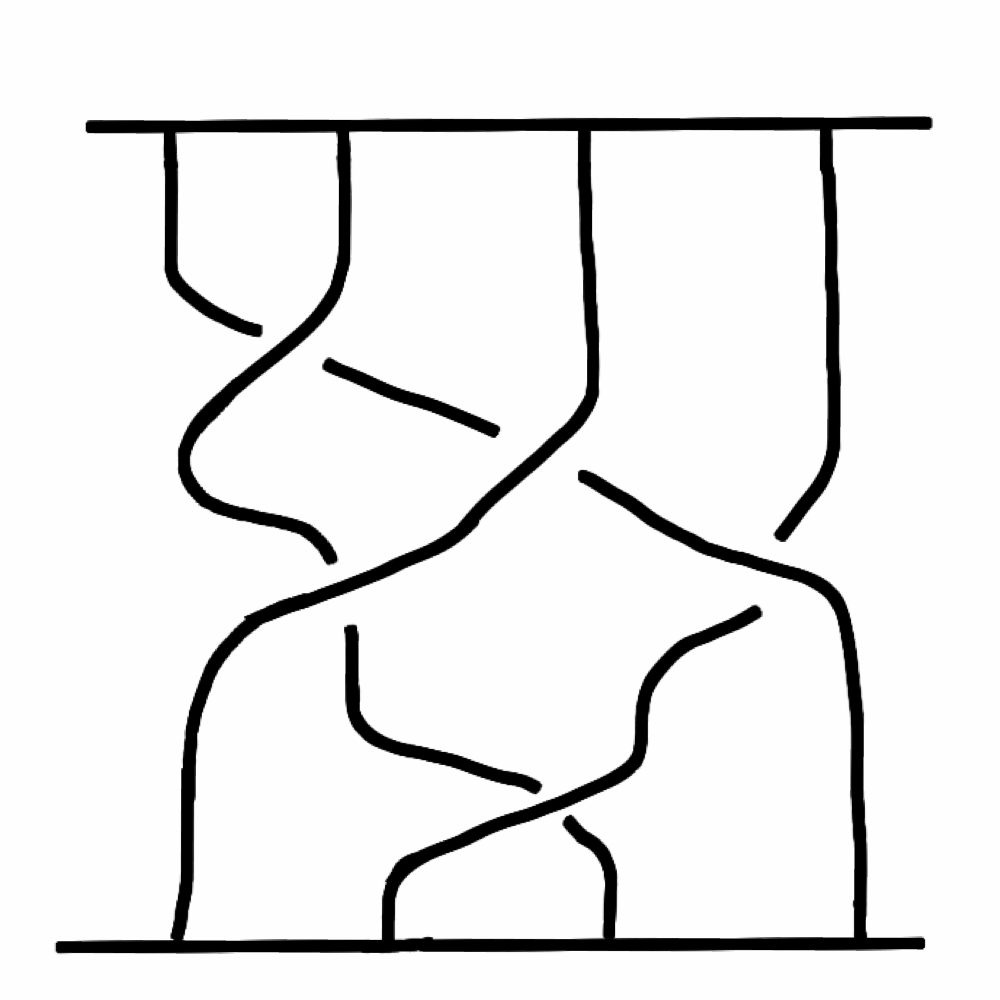
\includegraphics[width=\textwidth]{images/braid.png}
\end{subfigure}
\end{figure}



\end{document}